\documentclass[11pt,a4paper]{article}

% --- Encoding and fonts ---
\usepackage[utf8]{inputenc}
\usepackage[T1]{fontenc}
\usepackage{lmodern}

% --- Page layout ---
\usepackage[margin=1in]{geometry}
\usepackage{parskip}

% --- Math and symbols ---
\usepackage{amsmath}
\usepackage{amssymb}

% --- Tables and figures ---
\usepackage{booktabs}
\usepackage{tabularx}
\usepackage{graphicx}
\usepackage{float}

% --- Code listings ---
\usepackage{listings}
\usepackage{xcolor}

\lstset{
    basicstyle=\ttfamily\small,
    breaklines=true,
    frame=single,
    backgroundcolor=\color{gray!5},
    keywordstyle=\color{blue!70!black},
    commentstyle=\color{green!50!black},
    stringstyle=\color{red!60!black},
    showstringspaces=false
}

% --- Hyperlinks ---
\usepackage[hidelinks]{hyperref}

% --- Title metadata ---
\title{\textbf{Machine Learning-Based Crop Recommendation System}}
\author{Alusine Bah \\ \small Electrical \& Electronics Engineering \\ \small Islamic University of Technology (IUT), OIC}
\date{\today}

\begin{document}

\maketitle
\thispagestyle{empty}

\begin{abstract}
\noindent
Agriculture remains one of the most important sectors for sustaining human life, and the choice of the appropriate crop for a given plot of land is critical to maximizing productivity and minimizing waste. This project presents a machine learning-based Crop Recommendation System that predicts the most suitable crop to grow based on soil nutrient levels and climatic conditions. The system is trained on a dataset containing nitrogen (N), phosphorus (P), potassium (K), temperature, humidity, soil pH, and rainfall. Five classification algorithms were trained and compared: Logistic Regression, Decision Tree, Random Forest, K-Nearest Neighbors, and Support Vector Machine. The Random Forest classifier achieved the best performance, with a test accuracy of 99.32\%. The trained model was deployed as an interactive web application using Gradio, allowing users to enter soil and climate parameters and receive an instant crop recommendation.
\end{abstract}

\section{Introduction}

Agriculture is a central part of the economy of most nations. When deciding which crop to plant, farmers have traditionally relied on past experience and local knowledge. However, changing climate patterns and rising food demand have made it increasingly important to adopt modern, data-driven methods for agricultural decision-making.

Machine learning offers a practical solution for analyzing agricultural data and generating accurate predictions. This project develops a Crop Recommendation System that uses supervised learning to recommend the most suitable crop based on soil and environmental inputs.

\section{Problem Statement}

Farmers face several challenges when selecting which crop to grow:
\begin{itemize}
    \item Limited knowledge of soil nutrient composition.
    \item Uncertainty in weather conditions.
    \item Inefficient use of water and fertilizer.
    \item Reduced yield due to poor crop selection.
\end{itemize}

This project aims to build a system that analyzes soil and environmental data and returns accurate crop recommendations, reducing the guesswork involved in the decision.

\section{Objectives}

The main objectives of this project are:
\begin{enumerate}
    \item To build a machine learning model that predicts the most suitable crop from soil and climate inputs.
    \item To analyze the relationship between soil nutrients, climate parameters, and crop suitability.
    \item To improve agricultural decision-making through an accessible, easy-to-use interface.
\end{enumerate}

\section{Dataset Description}

The dataset used in this project contains the agricultural parameters that determine crop growth. Each row represents a specific combination of soil and environmental conditions, along with the recommended crop label.

\subsection{Features}
\begin{itemize}
    \item Nitrogen (N)
    \item Phosphorus (P)
    \item Potassium (K)
    \item Temperature ($^\circ$C)
    \item Humidity (\%)
    \item Soil pH
    \item Rainfall (mm)
\end{itemize}

\subsection{Target}
The target variable is the crop label --- the most appropriate crop to plant given the associated conditions. The dataset contains 22 distinct crop classes.

\subsection{Dataset Summary}
\begin{table}[H]
\centering
\begin{tabular}{lr}
\toprule
\textbf{Property} & \textbf{Value} \\
\midrule
Total records & 2{,}200 \\
Number of features & 7 \\
Number of classes & 22 \\
Samples per class & 100 \\
Missing values & 0 \\
\bottomrule
\end{tabular}
\caption{Summary of the dataset used in this project.}
\end{table}

The 22 crop classes are: rice, maize, chickpea, kidneybeans, pigeonpeas, mothbeans, mungbean, blackgram, lentil, pomegranate, banana, mango, grapes, watermelon, muskmelon, apple, orange, papaya, coconut, cotton, jute, and coffee.
\begin{figure}[H]
    \centering
    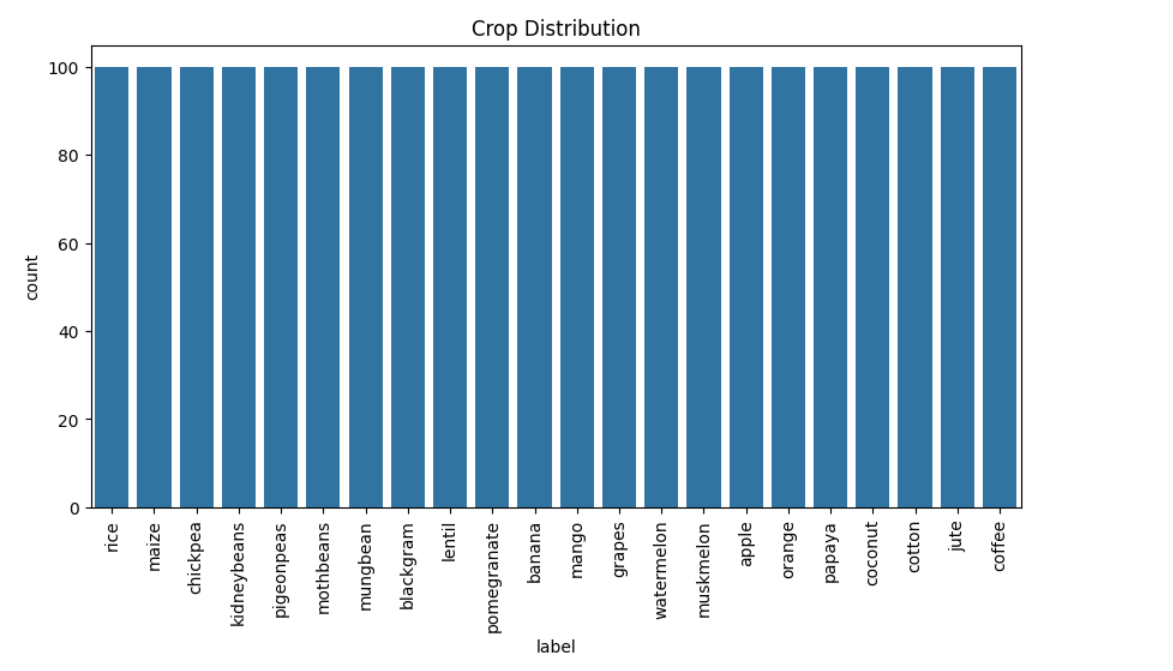
\includegraphics[width=0.9\textwidth]{crop_distribution.png}
    \caption{Distribution of samples across the 22 crop classes. Each class contains exactly 100 samples.}
    \label{fig:crop-distribution}
\end{figure}

\section{Methodology}

The project was carried out in a structured sequence of steps, from data loading to model deployment.

\subsection{Data Loading}
The dataset was loaded into Python using the Pandas library. Basic checks confirmed the shape, data types, and absence of missing values.

\subsection{Data Preprocessing}
\begin{itemize}
    \item Verified there were no missing values.
    \item Confirmed appropriate data types for all columns.
    \item Separated the input features ($X$) from the target variable ($y$).
    \item Applied \texttt{StandardScaler} to normalize feature ranges. The scaler was fit on the training set only, and then applied to the test set to avoid data leakage.
\end{itemize}

\subsection{Train-Test Split}
The dataset was divided into 80\% training data and 20\% test data using \texttt{train\_test\_split} with \texttt{random\_state=42}. This resulted in 1{,}760 training samples and 440 test samples.

\subsection{Model Training}
Five classification algorithms were trained and evaluated on the same split:
\begin{itemize}
    \item Logistic Regression (\texttt{max\_iter=5000})
    \item Decision Tree Classifier
    \item Random Forest Classifier
    \item K-Nearest Neighbors
    \item Support Vector Machine (RBF kernel)
\end{itemize}

\subsection{Model Evaluation}
Each model was evaluated using classification accuracy on the held-out test set. The best-performing model was selected for deployment.

\section{Model Selection}

Table~\ref{tab:results} summarizes the test accuracy obtained by each model.

\begin{table}[H]
\centering
\begin{tabular}{lc}
\toprule
\textbf{Model} & \textbf{Test Accuracy} \\
\midrule
Logistic Regression & 96.36\% \\
K-Nearest Neighbors & 95.68\% \\
Support Vector Machine & 96.82\% \\
Decision Tree & 98.86\% \\
\textbf{Random Forest} & \textbf{99.32\%} \\
\bottomrule
\end{tabular}
\caption{Comparison of model accuracies on the test set.}
\label{tab:results}
\end{table}

The Random Forest classifier achieved the highest accuracy. Its advantage over a single Decision Tree comes from bagging --- training many trees on different subsets of the data and averaging their predictions --- which reduces the variance to which a single tree is prone.

Based on these results, Random Forest was selected as the final model for the system.

\section{System Implementation}

The system was implemented in Python and developed in Google Colab. The implementation steps were:
\begin{enumerate}
    \item Load and explore the dataset.
    \item Preprocess the data and split into training and test sets.
    \item Train the five candidate models.
    \item Select the best-performing model.
    \item Build a prediction function around the trained model.
    \item Wrap the function in an interactive interface for end users.
\end{enumerate}

\section{System Interface}

A simple interactive interface was built using the Gradio library. The user enters seven numeric values:
\begin{itemize}
    \item Nitrogen
    \item Phosphorus
    \item Potassium
    \item Temperature
    \item Humidity
    \item Soil pH
    \item Rainfall
\end{itemize}

The trained model processes these values (after applying the same \texttt{StandardScaler}) and returns the recommended crop. The interface is designed to be usable without any technical background.
\begin{figure}[H]
    \centering
    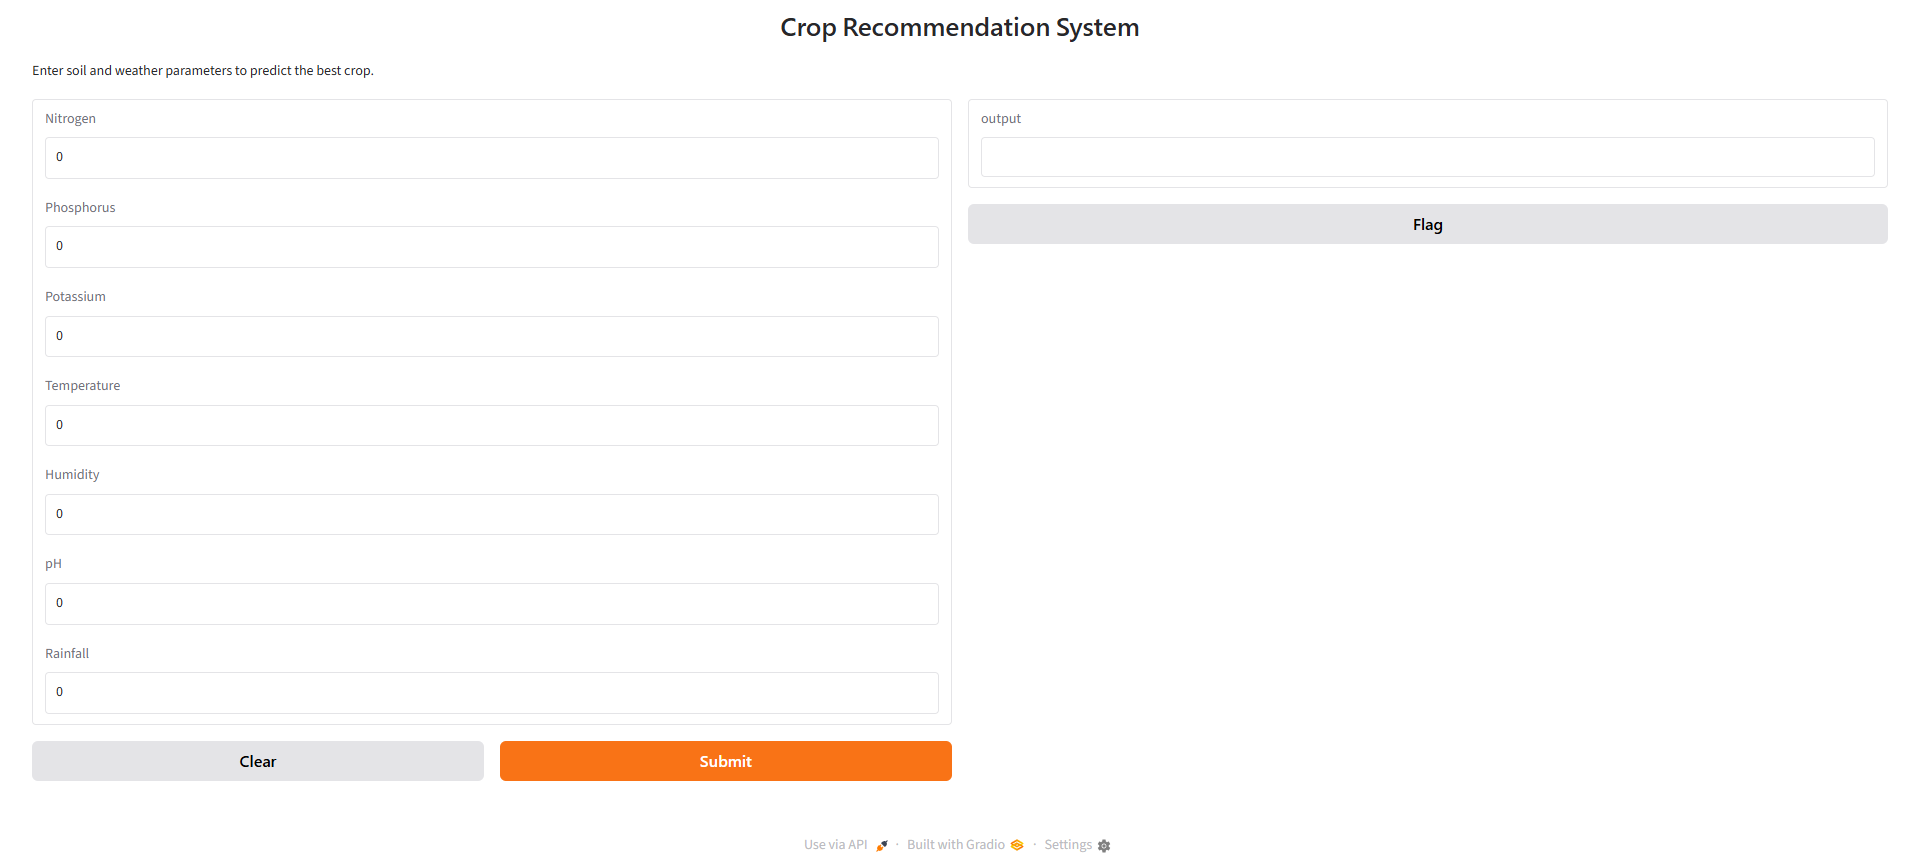
\includegraphics[width=0.85\textwidth]{gradio_form.png}
    \caption{The Gradio interface input form. The user enters seven soil and climate parameters.}
    \label{fig:gradio-form}
\end{figure}

\begin{figure}[H]
    \centering
    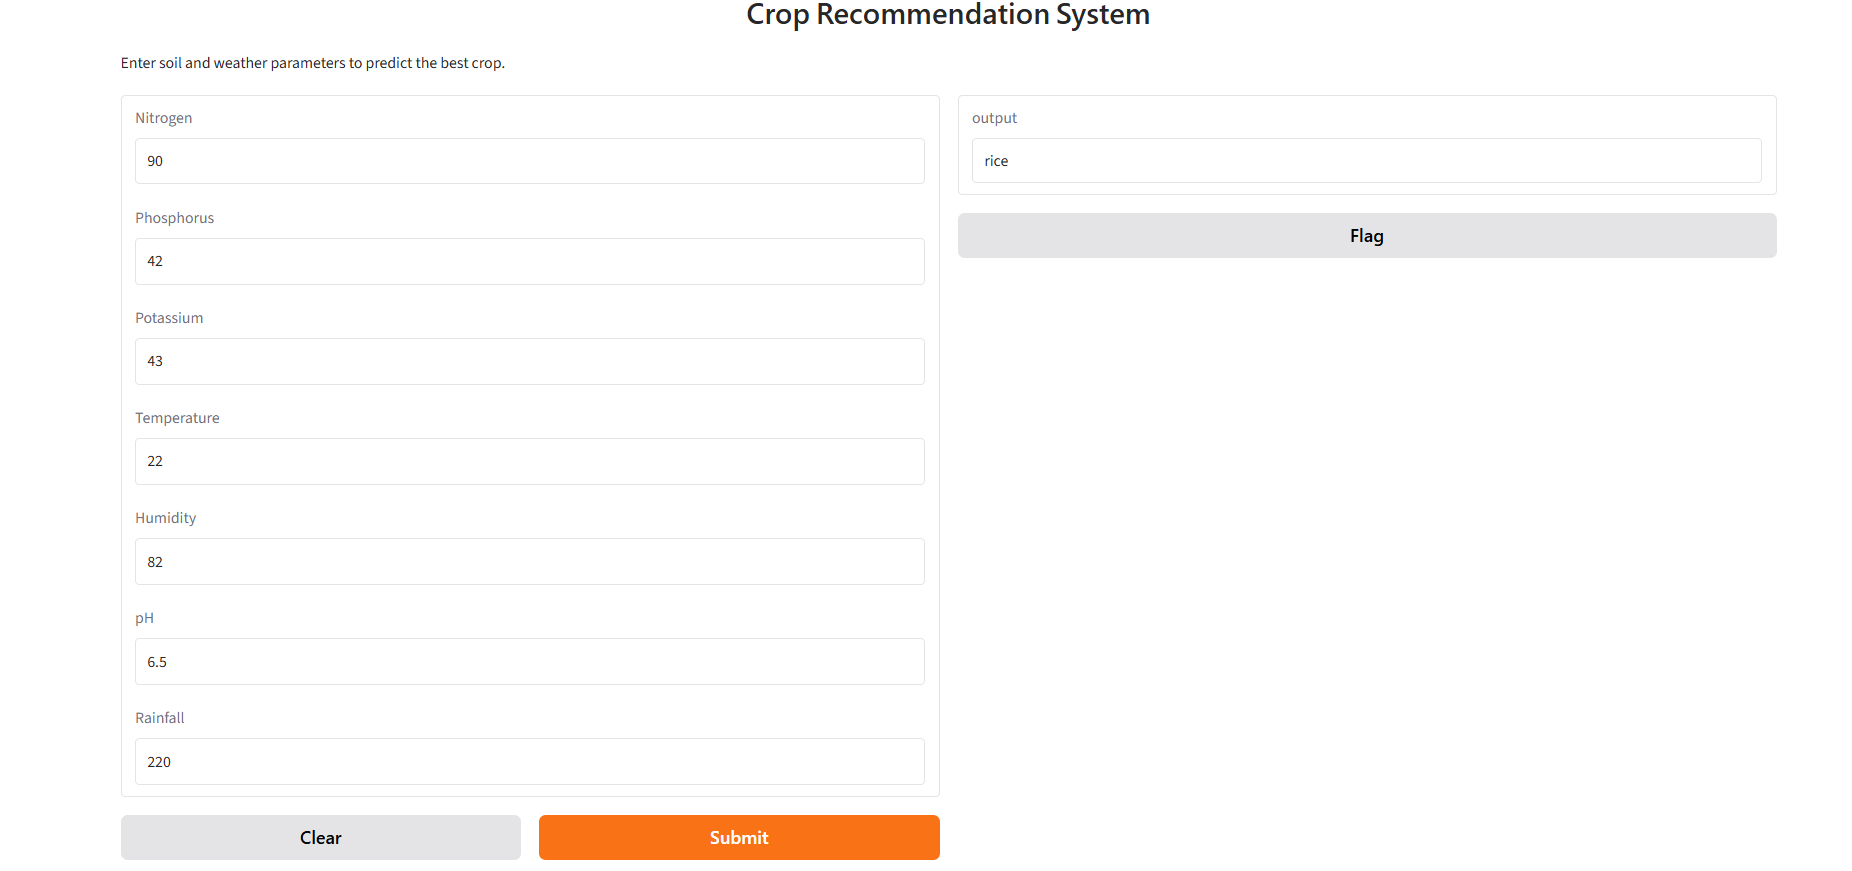
\includegraphics[width=0.85\textwidth]{gradio_output.png}
    \caption{The model returns the recommended crop \texttt{rice} for realistic rice-growing conditions.}
    \label{fig:gradio-output}
\end{figure}

\section{Results}

The system successfully predicts crops from the input parameters, with the Random Forest model producing reliable recommendations across all 22 classes. For example, given the inputs

\begin{center}
\texttt{N=90, P=42, K=43, temp=22, humidity=82, ph=6.5, rainfall=220}
\end{center}

the model returns \textbf{rice}, which is agronomically consistent with the warm, humid, high-rainfall conditions represented by those values.

\section{Advantages and Limitations}

\subsection*{Advantages}
\begin{itemize}
    \item Easy to use, with a clear input form and instant output.
    \item Fast predictions suitable for practical use.
    \item Removes reliance on guesswork in crop selection.
    \item Can contribute to improved agricultural productivity.
\end{itemize}

\subsection*{Limitations}
\begin{itemize}
    \item The quality of recommendations depends on the quality of the dataset.
    \item Weather data is not retrieved in real time --- values must be entered manually.
    \item Predictions are only reliable for inputs within the ranges seen during training.
    \item The model has not been validated on independent farm trials.
\end{itemize}

\section{Future Improvements}

Future work on this system could include:
\begin{enumerate}
    \item Integration of live weather data.
    \item Development of a mobile application.
    \item Expansion of the dataset with regional and seasonal variation.
    \item Exploration of more advanced machine learning and deep learning models.
    \item Support for multiple languages.
\end{enumerate}

\section{Conclusion}

The Crop Recommendation System demonstrates how machine learning can be effectively applied to agriculture. By analyzing soil nutrients and environmental conditions, the system provides accurate crop recommendations that can help farmers make better decisions, increase yields, and reduce waste. The project highlights the potential of data-driven methods to address real agricultural problems and to support sustainable farming practices.

\end{document}